%% *************************************************************************
%%
%% This is an RIT Space Exploration Standard defining guidelines for content
%% and formatting of project design documents.
%%
%% This document uses IEEEtran.cls, the official IEEE LaTeX class
%% for authors of the Institute of Electrical and Electronics Engineers
%% (IEEE) Transactions journals and conferences.
%%
%% *************************************************************************

%% *************************************************************************
% LaTeX REFERENCES
% ----------------
%   Intro to LaTeX: http://www.rpi.edu/dept/arc/docs/latex/latex-intro.pdf
%   Comprehensive LaTeX symbol list: http://tug.ctan.org/info/symbols/comprehensive/symbols-a4.pdf
%% *************************************************************************

% tell \LaTeX what kind of formatting to use
\documentclass[conference]{IEEEtran} % http://www.ctan.org/pkg/ieeetran
% enable placeholder text generator
\usepackage{blindtext}
% enable toolbox for embedding figures and pictures
\usepackage{graphicx}
% enable package for adding a list of variables and constants at the beginning, aka "nomenclature"
\usepackage{nomencl}
% enable package for easily formatting units
\usepackage{siunitx}
% enable package for cross-referencing figures, sections, references etc.
% how to use hyperref: http://www2.washjeff.edu/users/rhigginbottom/latex/resources/lecture09.pdf
\usepackage{hyperref}
% change text encoding to make it more crisp
\usepackage[T1]{fontenc}
% enable conditionals for help text
\usepackage{etoolbox}

\usepackage{float}

\usepackage{array}

\usepackage{booktabs}

\usepackage{tabularx}

% initialize nomenclature package
\makenomenclature{}

% set title. choose something as descriptive and precise as possible. Descriptive > sounding cool. remember this!
\title{Characterization of Habian Motion}


\author{
  % List the authors of the design document. The Champion should go first.
  % The \$~\$ markers tell \LaTeX{} to treat the text inside to be treated as a math expression. This way you can use operators like \textcaret{} to place characters as superscripts.
  % Some \LaTeX{} templates handle the author block in different ways. For example, the \href{http://www.worldscientific.com/worldscinet/jai}{Journal of Astronomical Instrumentation} requires the authors' addresses and emails to be included as well.
  % The \textbackslash{}thanks command puts the contents inside those brackets in a footnote at the bottom of the first page. Technically speaking, \textbackslash{}thanks is just a specially formatted footnote.
  % IEEE also has a ``long form'' author block for many authors. Check here for more information:
  % \url{https://tex.stackexchange.com/questions/156523/multiple-authors-with-common-affiliations-in-ieeetran-conference-template}
  % Read here for a more advanced options to modifying footnotes in the author block:  \url{http://tex.stackexchange.com/questions/826/symbols-instead-of-numbers-as-footnote-markers}
  %   Here, we use the IEEE long-form author block.
  \IEEEauthorblockN{% This block is for author Names.
    James~E~Parkus\IEEEauthorrefmark{1}
  }
  \IEEEauthorblockA{% This block is for the author Affiliations, aka department and university
    RIT Space Exploration, Rochester Institute of Technology \\ %\\ starts a new line
    Rochester, N.Y. \\
    Email:
    \IEEEauthorrefmark{1}jep7631@rit.edu
  }
  %%   Below, we use the short-form author block and basically hack it to suit our needs.
  % Philip~Linden$^{*\dagger}$%
  %   \thanks{$^{*}$Project Champion}%
  %   \thanks{$^{\dagger}$BS/MEng '17, Mechanical Engineering},
  % Austin~Bodzas$^{\ddagger}$%
  %   \thanks{$^{\ddagger}$BS '19, Computer Science},
  % Drew~Walters$^{\S}$%
  %   \thanks{$^{\S}$BS '18, Mechanical Engineering Technology},
  % T.J.~Tarazevits$^{**}$%
  %   \thanks{$^{**}$BS '19, Game Design \& Development}%

  %%   If there are many authors, consider using symbolic, numeric (aka arabic),  alphabet footnotes or a combination thereof.
  %% the recommended order for symbolic footnotes is
  %%   (1) asterisk        *   *
  %%   (2) dagger          †   \dagger
  %%   (3) double dagger   ‡   \ddagger
  %%   (4) section symbol  §   \S
  %%   et cetera. For higher counts, use 2x symbols (1)-(4) (i.e. (5) two asterisks **). Keep cycling through (1)-(4) using 3x, 4x, and so on.
  %%   Note that these symbol codes work in math mode and text mode.
  %%   There are ways to make LaTeX do this for you, but it is more advanced and not entirely necessary, especially for short author lists. Not worth the hassle, in my opinion.
}
% page header for pages other than cover page
\markboth{Project Design Document Standard}%
{Parkus \MakeLowercase{\textit{et al.}}: RIT Space Exploration}

% Initial setup is over, start building the document itself
\begin{document}
\maketitle%
% correct bad hyphenation here, separated by spaces
\hyphenation{explor-ation}

\begin{abstract}
The project, Habian Motion, is concerned with fully mapping the motion of a HAB during flight. The purpose is to understand the
forces, temperatures, wind, and pressures to which the HAB will be subjected. This will allow a further analysis of mechanical
and electrical components before launch to ensure the safety of the payload.

\end{abstract}

\label{sec:nomenclature}
\newcommand{\nomunit}[1]{%
\renewcommand{\nomentryend}{\hspace*{\fill}#1}}
\renewcommand{\nompreamble}{
    % If you include mathematical expressions or express variables in the design document, list them with their corresponding definitions here as a list.
    % The two lines below make it look nice when defining units/values to constants.

    % Note that math terms and non-math terms are separated and alphabetized, regardless of the order in which they are defined. (Recall terms \$like this\$ are in the math environment)
    % Read more about advanced nomenclature formatting here:\\
    % \url{https://www.sharelatex.com/learn/Nomenclatures}
  }
\nomenclature{RIT}{Rochester Institute of Technology}
\nomenclature{SPEX}{RIT Space Exploration}
\nomenclature{PDD}{Project Design Document}
\nomenclature{HAB}{High Altitude Balloon}
% Below are examples of using nomenclature for math symbols and constants or units
% \nomenclature{$\dot{m}$}{Mass flow rate
%   \nomunit{\,\si{\kilo\gram\per\second}}}
% \nomenclature{$c$}{Speed of light
%  \nomunit{\,\SI{2.9979e8}{\meter\per\second}}}
\printnomenclature{}

\section{Introduction}\label{sec:introduction}

\IEEEPARstart{T}{he} RIT SPEX HAB team has launched several HABs before. The overall missions, for the most part, have been successful; a successful takeoff, payload operation, and landing.
However, there have been a few errors that have caused problems for the payload, and specifically filming. The GoPro has yet to survive a full flight.
Unfortunately, the failure analysis is uncertain as the understanding of the conditions at the point of failure are unknown, thus it is difficult to
state the method of failure. This project will allow the team to collect a large amount of data which will be used to create a full map of the ambient conditions
of the HAB\@.

\section{Primary Objective}\label{sec:primary-obj}

The primary objective of the Characterization of Habian Motion is to create a conditional map of the entire flight. The data collection is vital. There
are several different events to be measured; ambient temperature, internal temperature, ambient pressure, internal pressure, rotation along the string axis,
the pendulum-like motion of the HAB, wind, and solar intensity.

The ambient and internal temperatures will assist in the understanding of thermal stress that may occur due to massive temperature fluctuation, in addition to
understanding how, exactly, the temperature changes with altitude. The ambient and internal pressures will allow the team to understand how the thermal diffusivity will change
over altitude, in addition to how the ambient and internal pressures differ to create a non-zero pressure differential. The string axis, along which the rotation is defined,
is an axial concentric line passing through the, theoretically, straight cable that connects the HAB to the balloon. The rotation is very important to understand because the
centripetal forces that ensue could be very high. These forces could causes severe mechanical and electrical problems. The pendulum-like motion of the HAB is very important because
it will set the standard for what cable is safe to use to connect the HAB to the balloon. The forces that the cable is subjected to have never been defined, due to the large amount of undefined
factors that could increase or decrease the tension. The wind and solar intensity are optional. They would be great to directly measure, however, if all the data is properly collected,
these events could be estimated to reasonable accuracy.

\begin{figure}
  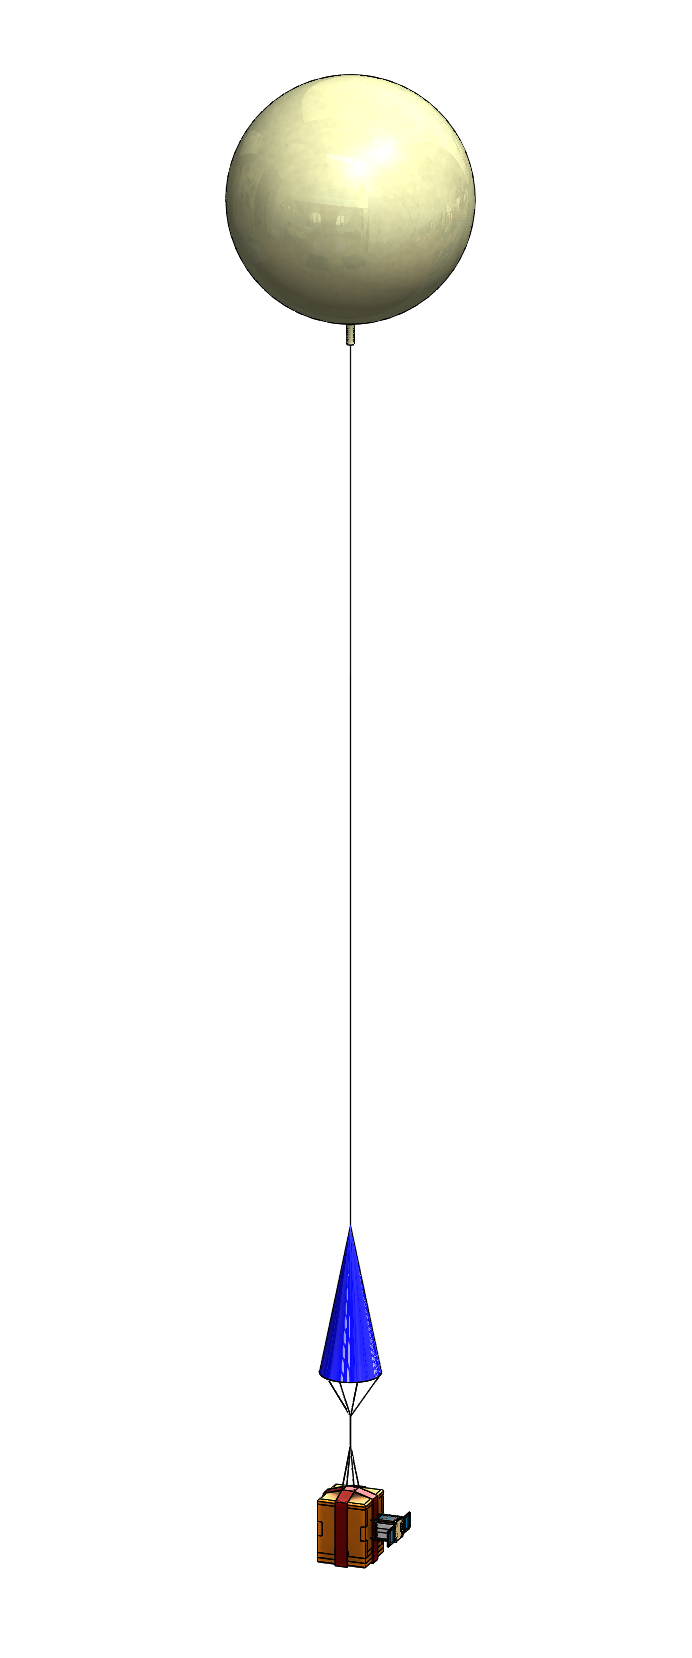
\includegraphics[width = \linewidth]{figs/full_HAB_model.png}
  \caption{This is the full proposed HAB model for the flight. The colors may vary.}
\end{figure}

\section{Benefit to SPEX}\label{sec:benefit}
The benefit to SPEX would be the product of the conditional map. The map could be open-sourced so any HAB team in the nation could use it for their specific needs. Even if their climate is
different, until they can perform the same data collection and analysis, this would be a great starting point for them. The SPEX HAB team would also gain great recognition for their work
and they would learn a great deal, from building and launching a HAB to performing complex data analysis and putting the results into a user-friendly map so that others could benefit from their
work.

\section{Implementation}\label{sec:implementation}
This project could possibly build off the horizon detection \& computer vision HAB project. The horizon detection would be a perfect method of collecting the sweep angle necessary to
calculate the pendulum-like motion of the HAB\@. The equation for this motion is below.

\begin{equation} \label{pendulum}
  \frac{d^2\theta}{dt^2} = -\frac{g}{l}\sin(\theta)
\end{equation}

Where; \(g\) is gravity, \(l\) is the length of the pendulum (in this case it would be the length of the cable), and \(\theta \) is the angle through which the pendulum moves, also known
as the sweep angle. The horizon detection payload will create a vector that spans the horizon. This will be called the horizon vector. The sweep angle is exactly equivalent to
the sweep angle of a vector normal to the horizon vector. This can be proven through simple geometry. This method would capture the sweep angle very well.

To collect the ambient and internal pressure and temperature data, the respective sensors will be placed on the outisde of the HAB and the inside. Because the HAB is made of
foam, threading sensors through to collect the necessary data should not be difficult. The rotational motion will also be captured through sensors, most likely are IMUs. They
are accurate and easy to implement.

\subsection{Deliverables}\label{subsec:deliverables}
  % When all is said and done, what will you have to show for it?
  % Examples: Hardware, software, poster, ImagineRIT demo, presentations, technical papers...
The deliverables for this project will be the full Habian motion map with the datasets used for the analysis. There will be a fully integrated system with the Computer Vision, Horizon Detection, and the CubeSat.
There will be a poster made for Imagine RIT explaining the detials of the mission, and if time permits, the map will be included. If the mission has not flown yet, a representative map will
be created in its stead to show visitors the primary goal of the mission. This project does include at minimum, 1 HAB launch. This will take place when the ground is in such a state that the
computer vision payload can perform its experiment. The ground must not be snow covered.

\subsection{Milestones}\label{subsec:milestones}
  % Be as detailed as you can, but it's okay if there are unknowns.
  % At the very least, specify how many semester you expect the project to take until it reaches completion.
The milestones for this project will be; finding the necessary sensors for measuring the rotation, temperatures, and pressures, determining whether or not it is feasible to measure
the solar intensity and wind, integrating the entire HAB payload, performing successful preliminary tests of the sensors, the flight, the data analysis, and the creation of the map.
A proposed timeline, for this project, is presented in \autoref{tab:proposed-timeline}.

\begin{table}\label{tab:proposed-timeline}
  \centering
  \begin{tabularx}{\columnwidth}{@{}cXc@{}}
    \multicolumn{2}{ c }{\textbf{Proposed Timeline}} \\ \toprule
    Week & Description \\ \midrule
    1 & Team Introductions and project planning \\
    2 & Sensor selection \\
    3 & System Mechanical Design and Analysis \\
    4 & Component level tests \\
    5 & Payload level tests \\
    6 & Payload integration \\
    7 & Payload integration \\
    8 & Full system tests \\
    9 & Launch Preperation \\
    10 & Launch \& Recovery \\
    11 & Data Collection and Organization \\
    12 & Data Analysis \\
    13 & Data Analysis \\
    14 & Creating Map \\
    15 & Finalizing Map \\
    \bottomrule
  \end{tabularx}
\end{table}

\section{Externalities}
  % Things not directly related to the work or outcomes, but related to the project as a whole.
\subsection{Prerequisite Skills}
  % Which skills do team members need to have before work can start (not including skills that will be learned ``on the job'')?
There are no prerequisites for this project. All necessary skills will be introduced and taught to a sufficient level. However, the recommended
skills are; MATLAB, structural analysis, electrical engineering, basic understanding of calculus, and a basic understanding of linear algebra. The
components used for capturing the data will require electrical engineering skills to integrate. The HAB itself must withstand certain forces to be
qualifed as flight-ready. MATLAB will be very important during the data analysis.

\subsection{Funding Requirements}
  % Estimate costs that would be needed to meet objectives.
An estimated budget for this project is \$300. The components for capturing the rotation, temperature, and pressure may need to be purchased. The
helium will need be pruchased and stored 1 week prior to the launch. Two cylinders of helium is required for appropriately filling the 1500 \(cm^3\) balloon.
Most of necessary mechanical components have been bought and others will be 3D printed. This leaves the rest of the budget to buy necessary, unforeseen components.

\subsection{Faculty Support}
Faculty support will be necessary to launch the HAB. They must file a NOTAM and apply for a launch permit that allows a HAB flight with a payload over 6 pounds. This permit
appies for a few months. That will most likely be the only faculty involvement. The rest of the HAB project is easily completed by a team of undergraduates, as history has shown.

\subsection{Long-Term Vision}
\label{sec:vision}
The long-term vision of this project is to increase chances of a successful flight by acknowledging the varying conditions of flight. Understanding the change in temperature and pressure over time
will be useful for understanding thermal stress that may arise. The rotation and pendulum forces will also assist in the understanding of mechanical stress on the outer shell, the foam,
and the cable that connects the HAB to the balloon. 

\section*{Acknowledgements}
The author would like to thank Dr.~Bill Destler and Rebecca Johnson for being exemplary humans, Anthony Hennig for founding RIT Space Exploration, and all the SPEX members that continue to invest their time and energy into the pursuit of space exploration.

\onecolumn
\appendices{}


\end{document}
